\documentclass[11pt]{article}

\usepackage[portuguese]{babel}
\usepackage[utf8]{inputenc}
\usepackage{amsmath}
\usepackage{graphicx}
\usepackage{float}
\usepackage{subfig}
\usepackage{fixltx2e}
\usepackage[bottom]{footmisc}
\usepackage{listings}
\usepackage{color} 
\usepackage[usenames,dvipsnames]{xcolor}
\usepackage[colorinlistoftodos]{todonotes}
\usepackage[font=footnotesize]{caption}

\setcounter{tocdepth}{3}

\numberwithin{equation}{section}

\linespread{1.3}
\usepackage{indentfirst}
\usepackage[top=2cm, bottom=2cm, right=2.3cm, left=2.3cm]{geometry}
\addto\captionsportuguese{\renewcommand{\contentsname}{Índice}}

\begin{document}

\begin{titlepage}
\begin{center}

\hfill \break
\hfill \break


\includegraphics[width=0.3\textwidth]{./logo}~\\[1cm] 

\textsc{\LARGE Instituto Superior Técnico}\\[0.25cm]
\textsc{\Large Mestrado Integrado em Engenharia Electrotécnica e de Computadores}\\[1.8cm]
\textsc{\huge Electrónica Rápida}\\[0.25cm]

\vspace{6mm}

{\huge \bfseries Projecto e Simulação de Amplificadores Lineares para Altas Frequências\\[1cm]}

\begin{tabular}{ l l }
Guilherme Branco Teixeira & \hspace{2mm} n.º 70214 \\
Maria Margarida Dias dos Reis & \hspace{2mm} n.º 73099 \\
Nuno Miguel Rodrigues Machado & \hspace{2mm} n.º 74236
\end{tabular}

\vspace{7mm}

Grupo n.º 2 de quarta-feira das 11h00 - 12h30

\vfill

{\large Lisboa, 25 de Abril de 2015} 

\end{center}
\end{titlepage}

\pagenumbering{gobble}
\clearpage

\tableofcontents
\pagebreak

\clearpage
\pagenumbering{arabic}

\section{Introdução}

O objectivo deste laboratório é estudar técnicas de projecto de amplificadores lineares de alta frequência, análise das suas características (estabilidade, ganho, adaptação e factor de ruído) e comportamentos. A caracterização dos dispositivos do amplificador será realizada através dos pârametros distribuídos - parâmetros S.

Utiliza-se um transístor da Hewlett-Packard (HP) ATF-35176, um transístor que utiliza tecnologia PHEMT (\textit{Pseudomorphic High Mobility Transistor}), preparado para trabalhar em altas frequências.

\section{Plano de Trabalhos}

As especificações do amplificador a construir podem ser consultadas na tabela seguinte, tal como as características do substrato plástico para alta-frequência da Taconic (TLY -3-0310-CH/CH), sobre qual o transístor irá ser implantado. 

\begin{table}[H]
	\centering
	\caption{Características do amplificador a projectar.}
	\vspace{-1.5mm}
	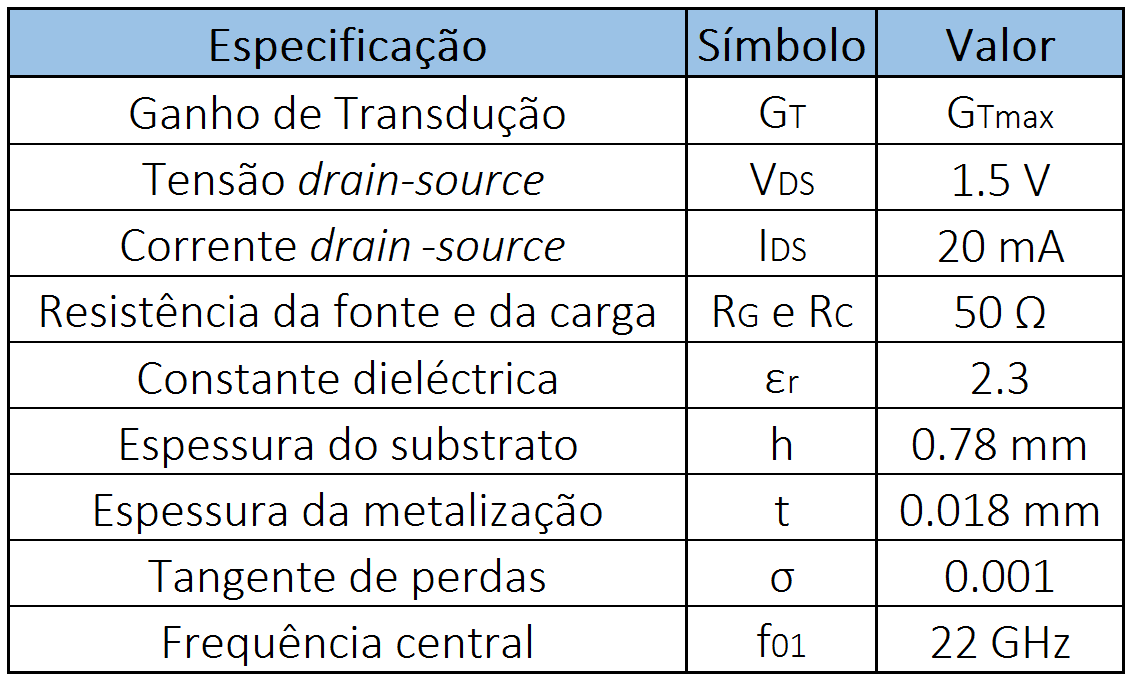
\includegraphics[keepaspectratio=true, scale=0.40]{teoricas/table1}
	\label{tab:car}
\end{table}

De notar que o valor da espessura do substrato foi modificado de 0.78 mm para 0.35 mm com o objectivo de garantir propagação transversal nas linhas de microfita, ou seja, garantir que estas têm um comprimento maior que a largura. 

Numa primeira fase do trabalho laboratorial é projectado e simulado o amplificador uniandar com linhas simétricas. Na segunda fase o amplificador é projectado com tecnologia de microfita.

\subsection{Projecto de um amplificador uniandar}

\subsubsection{a) Projecto do amplificador com linhas ideais}

Nesta primeira fase, o amplificador é constituído pelo transístor descrito anteriormente, no entanto, todos os dispositivos utilizados no seu projecto e simulação são dispositivos ideais.

\paragraph{PFR Pretendido} \hspace{0pt} 

Em primeiro lugar, é feita uma análise DC ao transístor que tem em vista obter o ponto de funcionamento em repouso (PFR) especificado. O circuito que nos permitiu alcançar essa análise é o que se vê na Figura \ref{fig:Circuito_0}.

\begin{figure}[H]
	\centering
	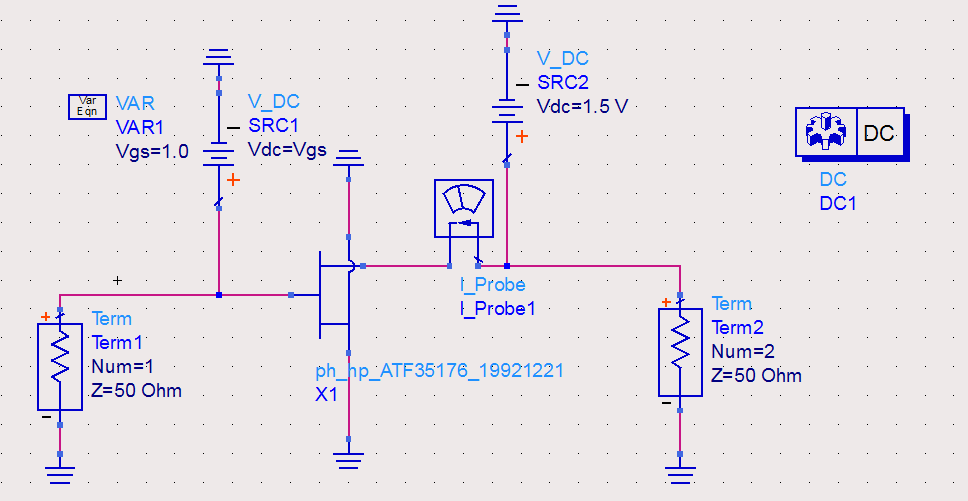
\includegraphics[keepaspectratio=true, scale=0.41]{exps/Circuito_0}
	\vspace{-0.5em}
	\caption{Circuito utilizado para obter o PFR desejado.}
	\label{fig:Circuito_0}
	\vspace{-0.8em}
\end{figure} 

A análise DC serve para descobrir o valor de $ V_{GS} $ correspondente ao PFR desejado. No circuito da Figura \ref{fig:Circuito_0} existe um componente denominado de \texttt{I\_Probe} que tem como objectivo controlar o valor de $ I_{D} $ à medida que o valor de $ V_{GS} $ varia. Um excerto dos resultados desta análise pode ser consultado na Figura \ref{fig:VGS}, onde se pode concluir que o valor da tensão  $V_{GS}$ que melhor corresponde a uma corrente $I_{D}$ de $20$ mA ($20.03$ mA) é de $-0.277$ V.

\begin{figure}[H]
	\centering
	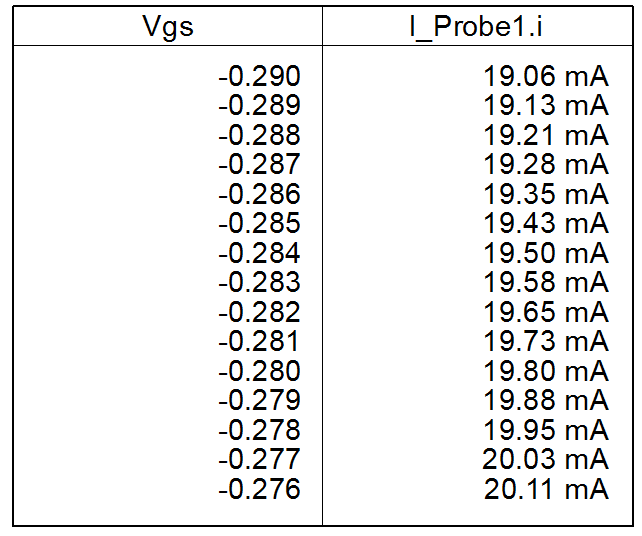
\includegraphics[keepaspectratio=true, scale=0.27]{exps/Vgs}
	\vspace{-0.5em}
	\caption{Valores de $V_{GS}$ correspondentes à corrente de \texttt{I\_Probe}.}
	\label{fig:VGS}
	\vspace{-0.8em}
\end{figure} 

\paragraph{Análise em Alta-Frequência} \hspace{0pt} 

Com o transístor a funcionar no PFR desejado, é preciso construir um novo circuito que contenha condensadores e bobines ideais, \texttt{DC\_Block} e \texttt{DC\_Feed}, respectivamente, para que seja possível realizar a simulação dos parâmetros S. Este circuito apresenta-se de seguida.

\begin{figure}[H]
	\centering
	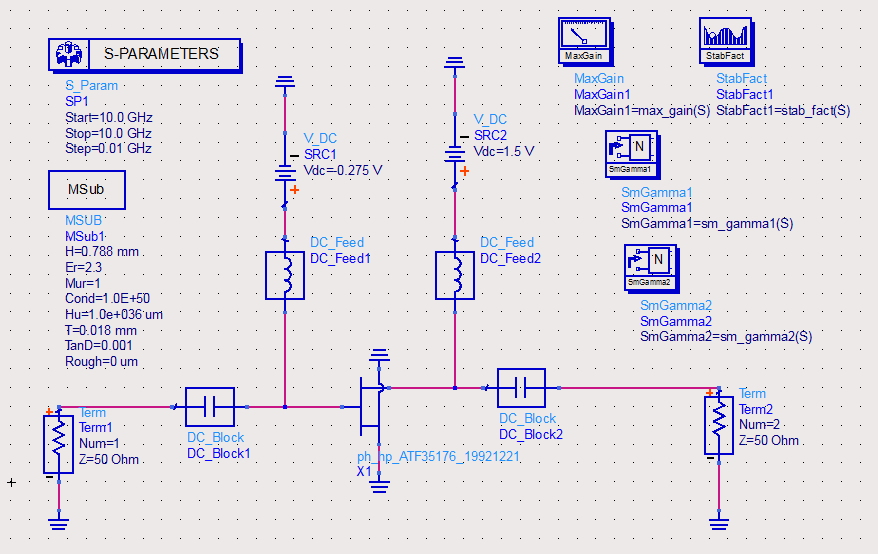
\includegraphics[keepaspectratio=true, scale=0.41]{exps/Circuito_1}
	\vspace{-0.5em}
	\caption{Circuito utilizado para obter o valores dos parâmetros S.}
	\label{fig:Circuito_1}
	\vspace{-0.8em}
\end{figure}

Simulando o circuito anteriormente projectado foram obtidos os seguintes valores para os parâmetros S, K (parâmetro de estabilidade), MAG (\textit{maximum available gain}) e para as cargas de adaptação para o transístor à frequência central.

\begin{table}[H]
 	\centering
 	\caption{Parâmetros que definem o transístor.}
 	\vspace{-1.5mm}
 	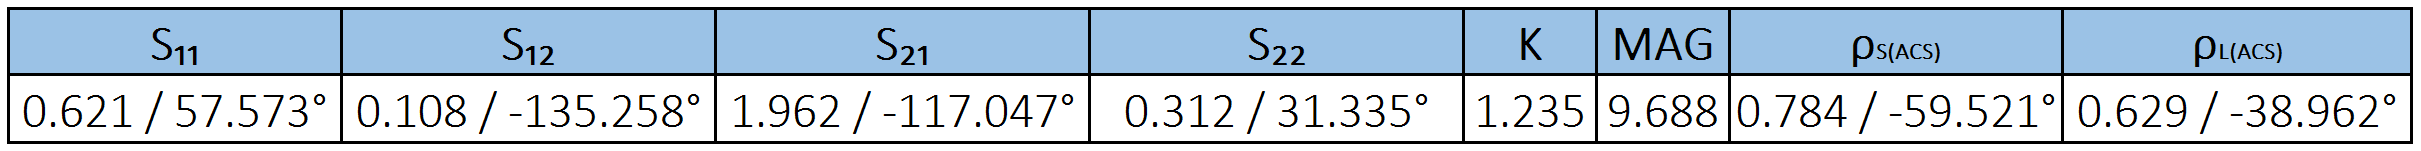
\includegraphics[keepaspectratio=true, scale=0.45]{teoricas/table2}
\end{table}

De notar que os valores obtidos experimentalmente para os parâmetros S não podem ser verificados na \textit{datasheet} do transístor, uma vez que esta apenas especifica o comportamento do ATF-35176 para frequências entre 2 GHz e 18 GHz.

Com os valores da Tabela 2 determinados pode-se calcular o valor de $\Delta$, ou seja, o determinante da matriz de dispersão:

\vspace{-3mm}
\begin{equation}
\Delta = S_{11}S_{22} - S_{21}S_{12} = 0.067\angle-7.24 ^{\circ}.
\label{eq:delta}
\end{equation}

\vspace{1mm} 
Como se pode ver, K $= 1.236 > 1$, $\lvert \Delta \rvert = 0.067 < 1$ e $\lvert S_{ii} \rvert < 1$, pelo que o transístor é incondicionalmente estável.s

\paragraph{Projecção da Malha de Entrada e de Saída} \hspace{0pt} 

Optou-se por projectar a malha de entrada e de saída com a Carta de Smith, recorrendo ao ADS. Como K $ > 1$ é possível efectuar adaptação conjugada simultânea (ACS) e, como se pretende adicionar elementos às malhas sabe-se que:

\vspace{-3mm}
\begin{equation}
\rho_{\text{in}} = \rho_{\text{S}}^{*} ~~ \text{e} ~~ \rho_{\text{out}} = \rho_{\text{L}}^{*}.
\end{equation}

\vspace{1mm} 
O circuito com malhas de adaptação é apresentado de seguida.

\begin{figure}[H]
	\centering
	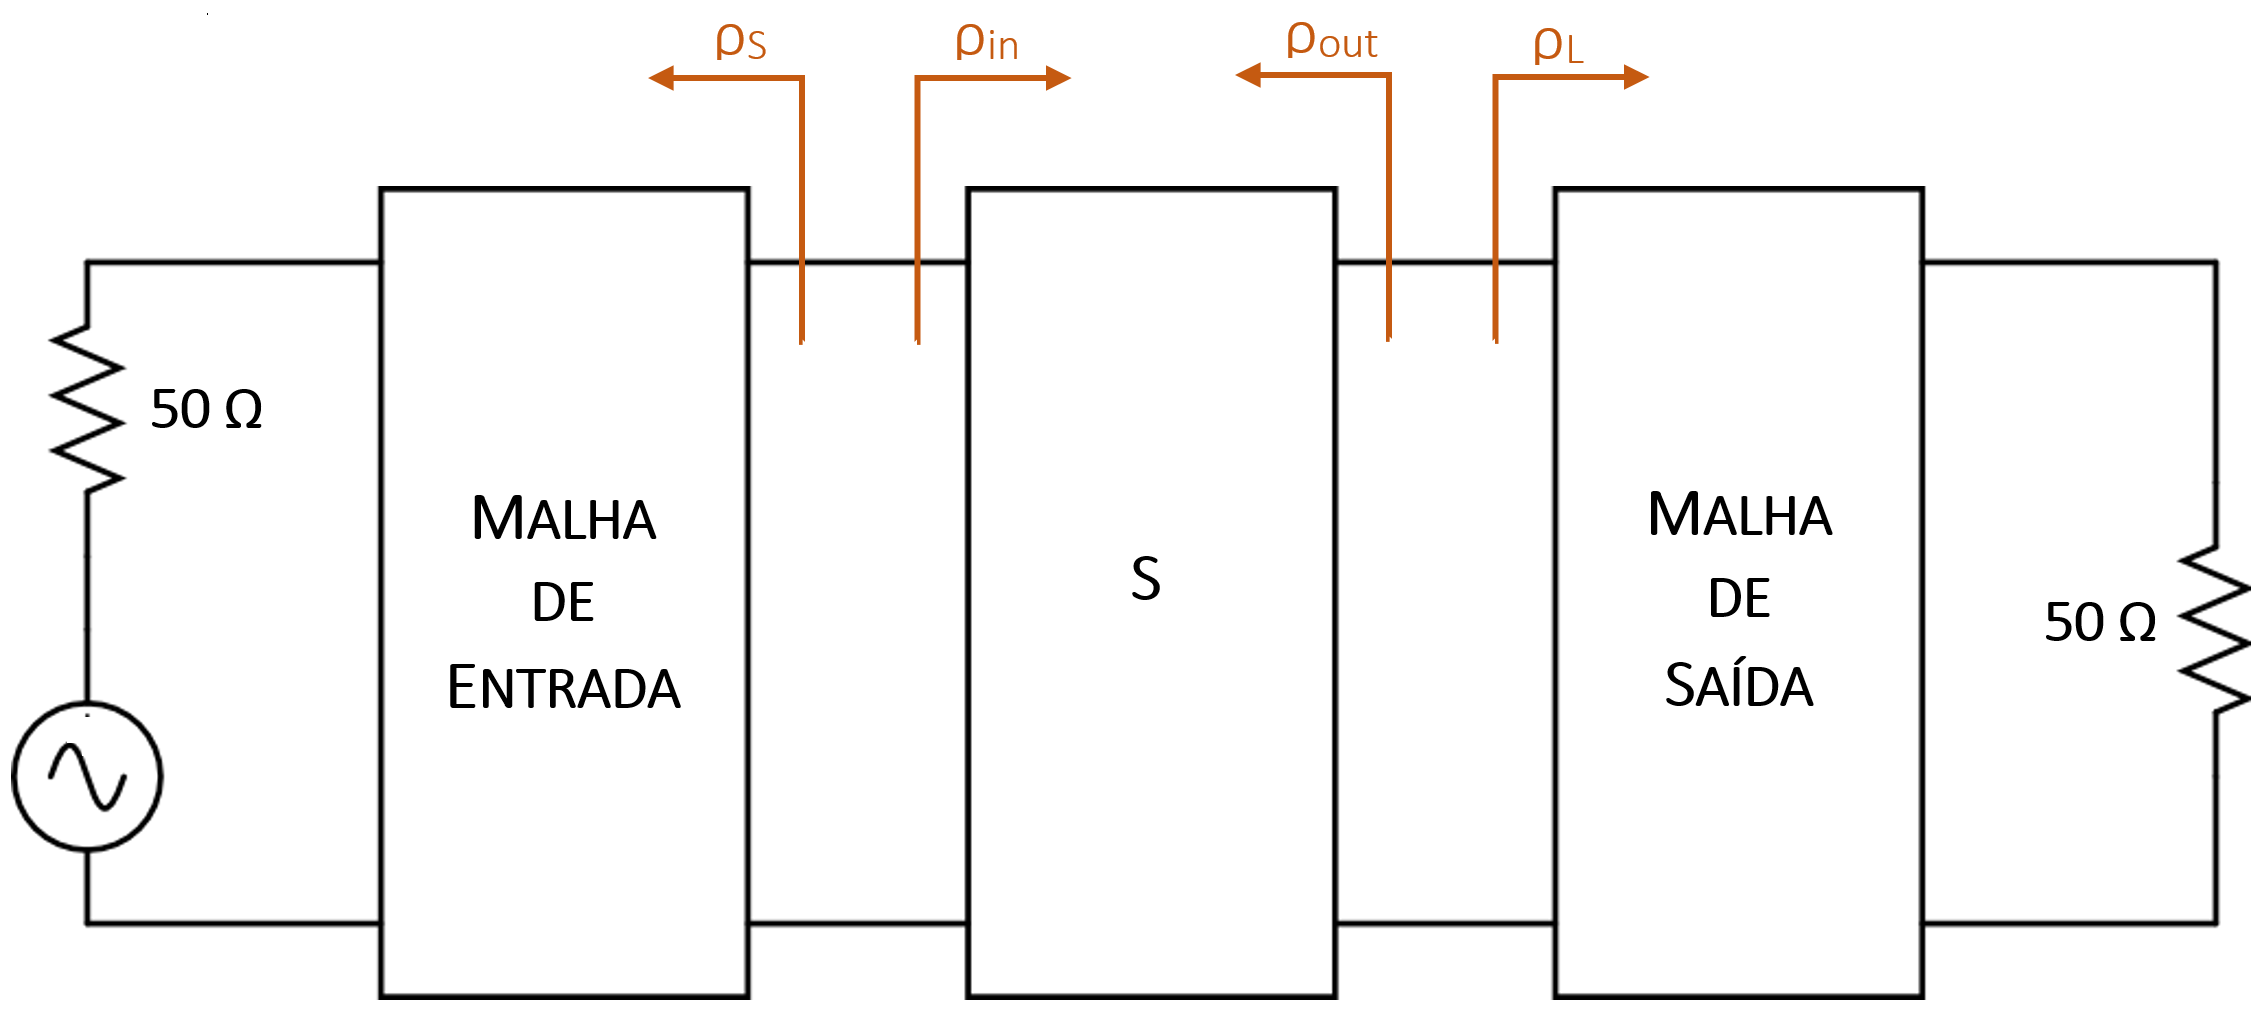
\includegraphics[keepaspectratio=true, scale=0.35]{teoricas/malhas}
	\vspace{-0.5em}
	\caption{Circuito que inclui as malhas de adaptação à entrada e à saída.}
	\vspace{-0.8em}
\end{figure}

Começando pela malha de entrada, ou seja, pelo gerador e sabendo que a malha de adaptação é do tipo linha-\textit{stub}, o circuito que se pretende projectar é da seguinte forma.

\begin{figure}[H]
	\centering
	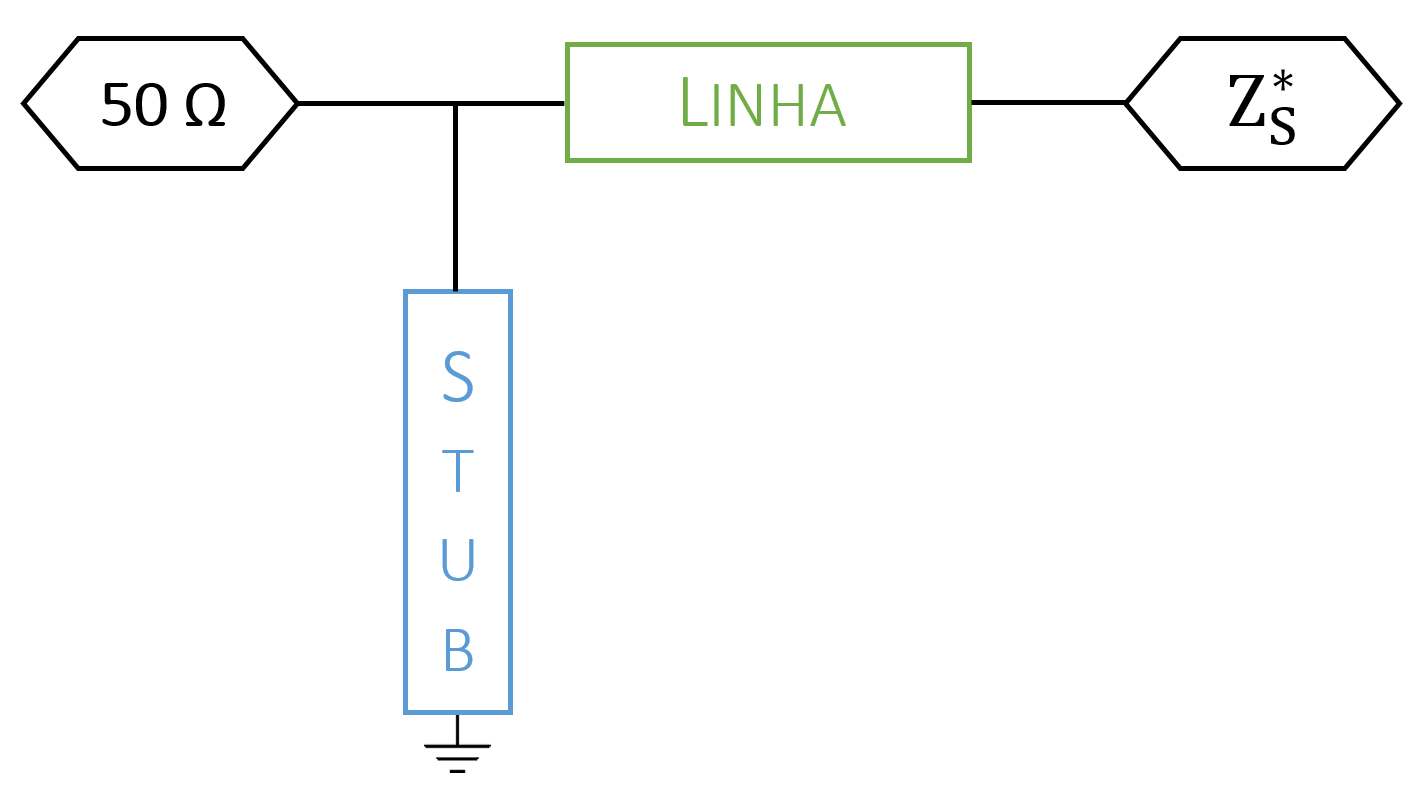
\includegraphics[keepaspectratio=true, scale=0.25]{teoricas/malhaentrada}
	\vspace{-0.5em}
	\caption{Malha de adaptação de entrada.}
	\vspace{-0.8em}
\end{figure}

Esta malha é construída com a adição de elementos, ou seja, \textit{towards generator}. O valor de $Z_{\text{S}}^{*}$ é de $0.784\angle59.529 ^{\circ}$.

No ADS, com recurso à Carta de Smith, determinou-se o comprimento eléctrico da linha de entrada, $\theta_{\text{L}_{\text{in}}}$, e o comprimento eléctrico do \textit{stub}, $\theta_{\text{S}_{\text{in}}}$. 

\begin{figure}[H]
	\centering
	\includegraphics[keepaspectratio=true, scale=0.45]{exps/Gerador_cc_line}
	\vspace{-0.5em}
	\caption{Determinação do comprimento eléctrico da linha de entrada - situação de CC.}
	\vspace{-0.8em}
\end{figure}

\begin{figure}[H]
	\centering
	\includegraphics[keepaspectratio=true, scale=0.45]{exps/Gerador_cc_stub}
	\vspace{-0.5em}
	\caption{Determinação do comprimento eléctrico do \textit{stub} de entrada - situação de CC.}
	\vspace{-0.8em}
\end{figure}

\vspace{-3mm}
\begin{equation}
	\theta_{\text{L}_{\text{in}}} = 100.494^{\circ}  ~~ \text{e} ~~ \theta_{\text{S}_{\text{in}}} = 21.751^{\circ}.
\end{equation}

\vspace{1mm} 
É de notar que os valores determinados anteriormente são para o \textit{stub} terminado em curto-circuito (CC), pois é nessa situação que o \textit{stub} é menor, tal como pretendido. Para verificar, optou-se por projectar a malha de entrada para o \textit{stub} terminado em circuito-aberto (CA).

\begin{figure}[H]
	\centering
	\includegraphics[keepaspectratio=true, scale=0.45]{exps/Gerador_Ca_line}
	\vspace{-0.5em}
	\caption{Determinação do comprimento eléctrico da linha de entrada - situação de CA.}
	\vspace{-0.8em}
\end{figure}

\begin{figure}[H]
	\centering
	\includegraphics[keepaspectratio=true, scale=0.45]{exps/Gerador_Ca_stub}
	\vspace{-0.5em}
	\caption{Determinação do comprimento eléctrico do \textit{stub} de entrada - situação de CA.}
	\vspace{-0.8em}
\end{figure}

Como se pode ver, para este caso o \textit{stub} é maior e, como tal, não é a solução preferível.

Olhando agora para a malha de saída, ou seja, para a carga e sabendo que a malha de adaptação é do tipo linha-\textit{stub}, o circuito que se pretende projectar é da seguinte forma.

\begin{figure}[H]
	\centering
	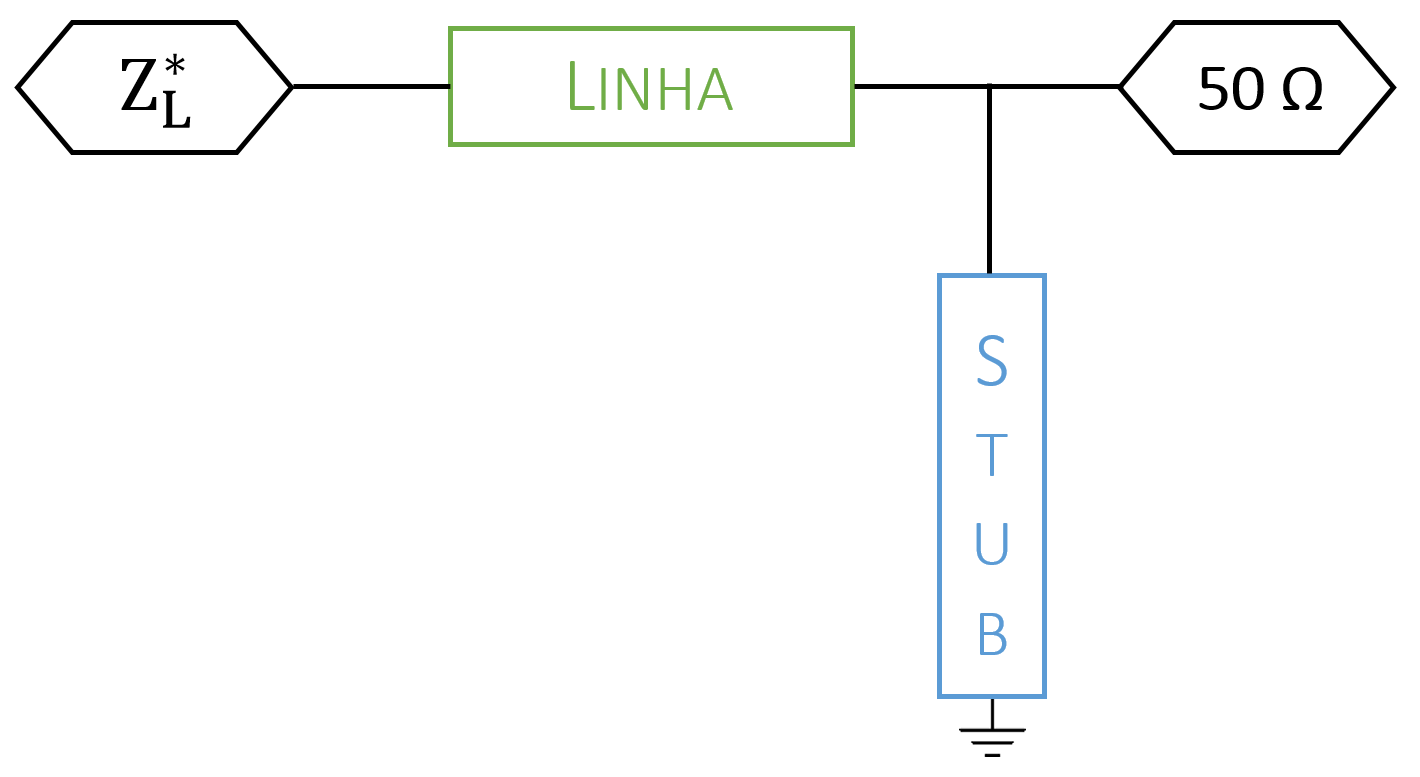
\includegraphics[keepaspectratio=true, scale=0.25]{teoricas/malhasaida}
	\vspace{-0.5em}
	\caption{Malha de adaptação de saída.}
	\vspace{-0.8em}
\end{figure}

Esta malha é construída com a adição de elementos, ou seja, \textit{towards generator}. O valor de $Z_{\text{L}}^{*}$ é de $0.628\angle39.020 ^{\circ}$.

No ADS, com recurso à Carta de Smith, determinou-se o comprimento eléctrico da linha, $\theta_{\text{L}_{\text{out}}}$, e o comprimento eléctrico do \textit{stub}, $\theta_{\text{S}_{\text{out}}}$. 

\begin{figure}[H]
	\centering
	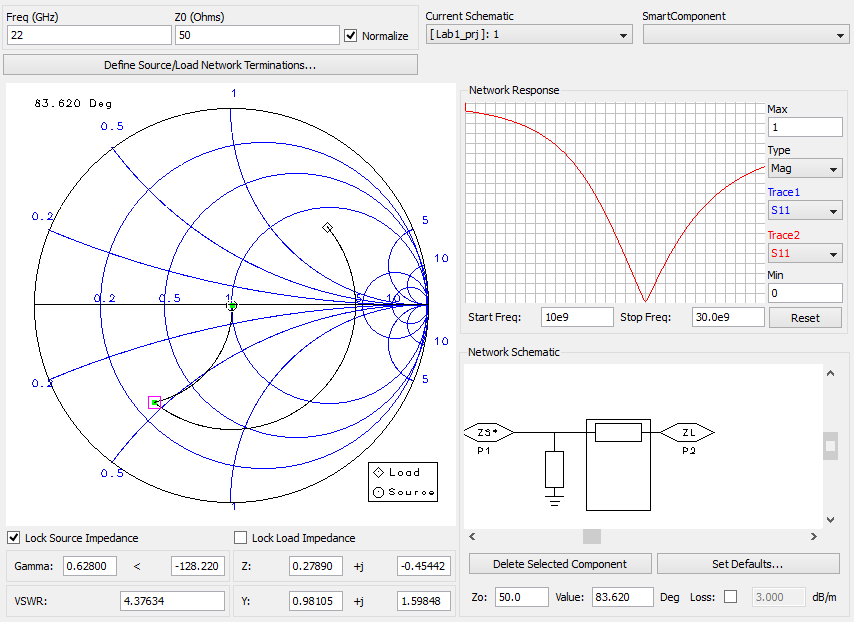
\includegraphics[keepaspectratio=true, scale=0.45]{exps/Carga_CC_line}
	\vspace{-0.5em}
	\caption{Determinação do comprimento eléctrico da linha de saída - situação de CC.}
	\vspace{-0.8em}
\end{figure}

\begin{figure}[H]
	\centering
	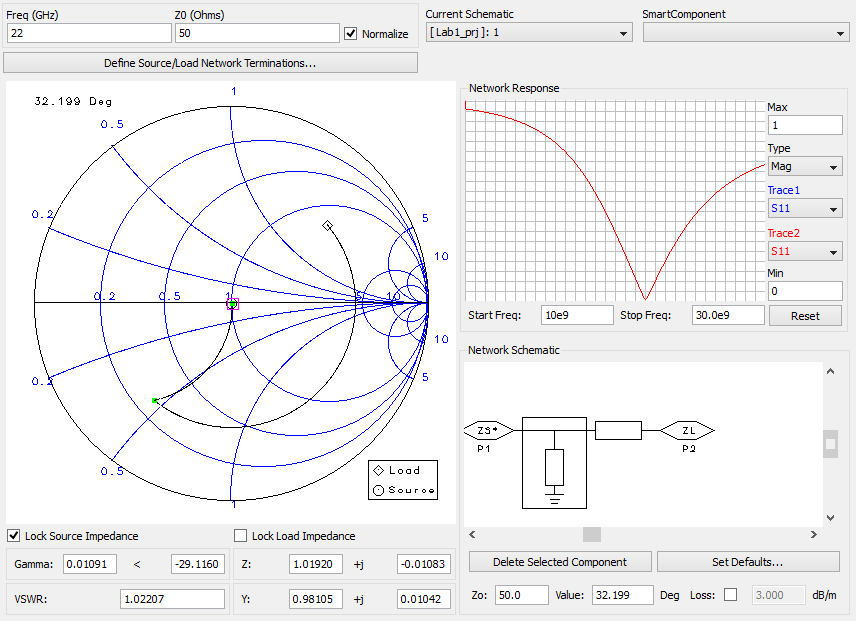
\includegraphics[keepaspectratio=true, scale=0.45]{exps/Carga_CC_stub}
	\vspace{-0.5em}
	\caption{Determinação do comprimento eléctrico do \textit{stub} de saída - situação de CC.}
	\vspace{-0.8em}
\end{figure}

\vspace{-3mm}
\begin{equation}
\theta_{\text{L}_{\text{out}}} = 83.620^{\circ}  ~~ \text{e} ~~ \theta_{\text{S}_{\text{out}}} = 32.199^{\circ}.
\end{equation}

\vspace{1mm} 

\paragraph{Simulação do Amplificador Ideal} \hspace{0pt}  

Após obtermos os valores dos comprimentos eléctricos dos dispositivos que compõem as malhas de adaptação de entrada e saída através do ADS, poderemos então projectar um amplificador com malhas ideais compostas por dispositivos sem perdas. O circuito projectado pode ser observado na Figura \ref{fig:circ_ideal}.

\begin{figure}[H]
	\centering
	\includegraphics[keepaspectratio=true, scale=0.45]{exps/Circuito_ideal}
	\vspace{-0.5em}
	\caption{Circuito do Amplificador com linhas ideais.}
	\vspace{-0.8em}
	\label{fig:circ_ideal}
\end{figure}
 
Após o circuito estar montado, as linhas ideais com os seus comprimentos eléctricos e com frequência de referência centrada nos $ 22 GHz $, foram realizadas várias simulações numa banda de frequências que compreende entre $ 10 GHz $ a $ 30GHz $ de modo a obter os parâmetros pedidos, tal como se pode observar nas Figuras \ref{fig:ideal_estavel}, \ref{fig:ideal_S} e \ref{fig:ideal_noise}.

Em primeiro lugar iremos testar a estabilidade do circuito, estabilidade esta que,teoricamente, já tinha sido garantida com a Equação \ref{eq:delta}. Tal como se pode ver na Figura \ref{fig:ideal_estavel}, a variável de estabilidade apresenta sempre valores superiores a zero, o que confirma a estabilidade do amplificador na banda de $ 10 GHz $ a $ 30GHz $.

\begin{figure}[H]
	\centering
	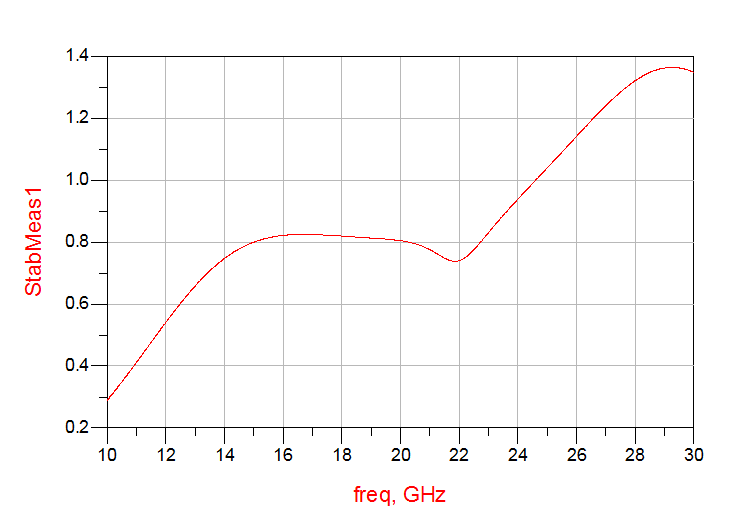
\includegraphics[keepaspectratio=true, scale=0.45]{exps/Ideal_estab}
	\vspace{-0.5em}
	\caption{Estabilidade do Amplificador com linhas ideais.}
	\vspace{-0.8em}
	\label{fig:ideal_estavel}
\end{figure}

Através da simulação foi possível obter os Parâmetros-S, sendo que a parcela S(1,2) não representa uma caracteristica relevante no nosso amplificador, e por isso não foi projectada. Ao observar a Figura \ref{fig:ideal_S}, e tendo em conta que a parcela S(1,1) representa o factor de reflexão à entrada, S(2,2) representa o factor de reflexão na saída e S(2,1) representa o ganho de transdução.

\begin{figure}[H]
	\centering
	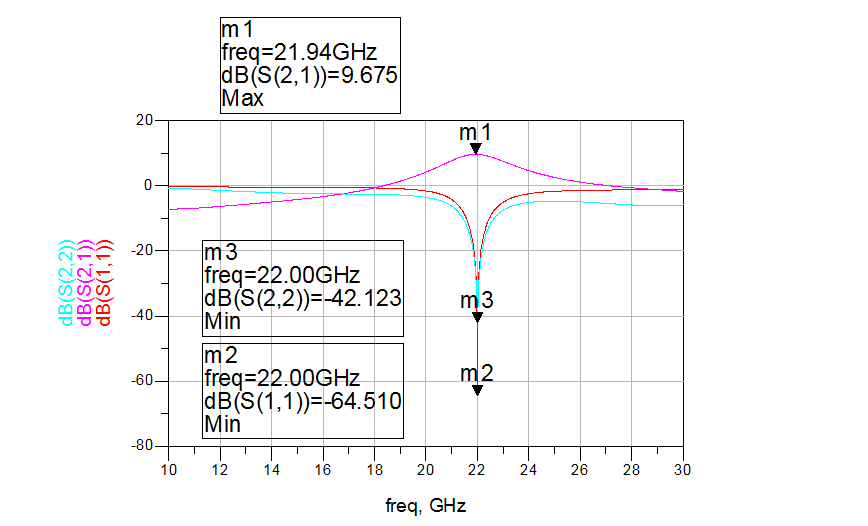
\includegraphics[keepaspectratio=true, scale=0.45]{exps/Ideal_S}
	\vspace{-0.5em}
	\caption{Parâmetros-S do Amplificador com linhas ideais.}
	\vspace{-0.8em}
	\label{fig:ideal_S}
\end{figure}

Foi também possível medir o \textit{noise} do amplificador ao longo da banda, e mais especificamente na frequência de referência sobre a qual o amplificador irá operar, tal como se pode observar na Figura \ref{fig:ideal_noise}.

\begin{figure}[H]
	\centering
	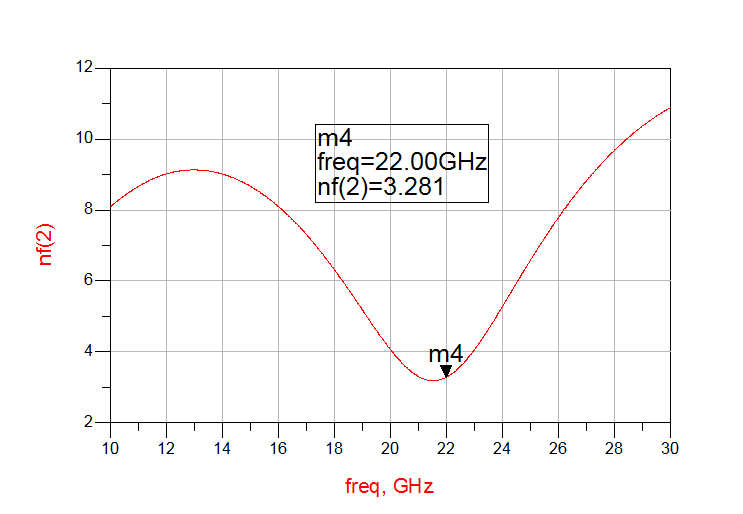
\includegraphics[keepaspectratio=true, scale=0.45]{exps/Ideal_noise}
	\vspace{-0.5em}
	\caption{\textit{Noise} no Amplificador com linhas ideais.}
	\vspace{-0.8em}
	\label{fig:ideal_noise}
\end{figure}


\todo{Margarida se quiseres passa estes valores para uma tabela, deve ser mais bonito}

Tendo obtido os seguintes resultados da simulação:
\begin{list}{-}{}
	\item Ganho de transdução =$ 9.625 dB $;
	\item Factor de reflexão à entrada =$ -64.510 dB $;
	\item Factor de reflexão na saída =$ -42.123 dB $;
	\item \textit{noise} =$ 3.281 $;
\end{list}

\todo{Tirar conclusões sobre isto, mas poucas isto é tipo a experiência base, o ideal, se calhar explicava-se o que significa cada coisa}


\subsubsection{b) Projecto do amplificador utilizando tecnologia microfita}

Tendo já completado o projecto do amplificador com linha ideais, temos agora as características ideais que representam um objectivo que tentaremos alcançar, mas que no entanto o máximo que se pode aspirar é chegar o mais perto possível, pois no caso ideal não foram consideradas qualquer tipo de perdas.

Em primeiro lugar os blocos \texttt{DC\_Block} e \texttt{DC\_Feed} terão de ser substituídos por dispositivos reais com valores reais (condensadores e bobines respectivamente). 

\todo{O Gui ainda vai espectar aqui as expressões que utilizou para calcular C e L}

Em segundo lugar teremos de substituir as linhas ideais por dispositivos reais, dispositivos estes que representam a tecnologia microfita utilizada no amplificador. Para tal objectivo será utilizado a ferramenta do ADS, \texttt{LineCalc}, como se pode ver na Figura \ref{fig:LineCalc}, para calcular as dimensões das microfitas a utilizar é necessário colocar as características do nosso substrato (Tabela \ref{tab:car}), a frequência de referência e finalmente a impedância e comprimento eléctrico desejados para a microfita.

\begin{figure}[H]
	\centering
	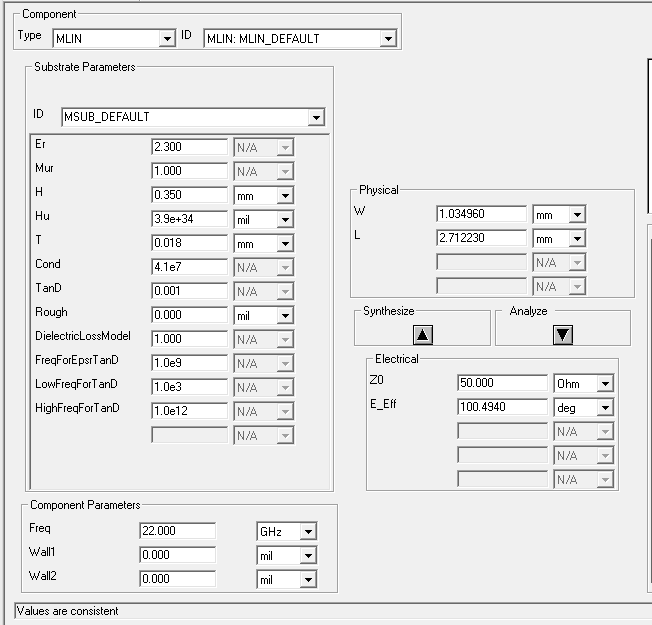
\includegraphics[keepaspectratio=true, scale=0.45]{exps/LineCalc}
	\vspace{-0.5em}
	\caption{exemplo de \texttt{LineCalc}.}
	\vspace{-0.8em}
	\label{fig:LineCalc}
\end{figure}

Numa primeira fase, as malhas de adaptação foram construídas com os elementos \texttt{MLIN}(linhas) e \texttt{MLSC}(stubs), o circuito que se obteve está representado na Figura \ref{fig:mf_stub_circuito} e os seus parametros-S podem ser observados na Figura \ref{fig:mf_stub_S}.

\begin{figure}[H]
	\centering
	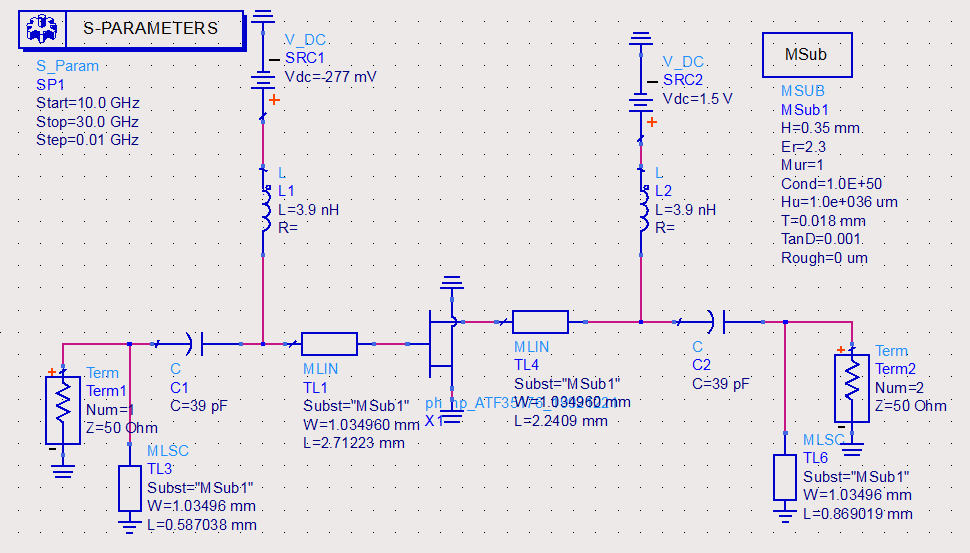
\includegraphics[keepaspectratio=true, scale=0.45]{exps/Circuito_mf_stub}
	\vspace{-0.5em}
	\caption{Circuito com microfitas, linhas e stubs.}
	\vspace{-0.8em}
	\label{fig:mf_stub_circuito}
\end{figure}

\begin{figure}[H]
	\centering
	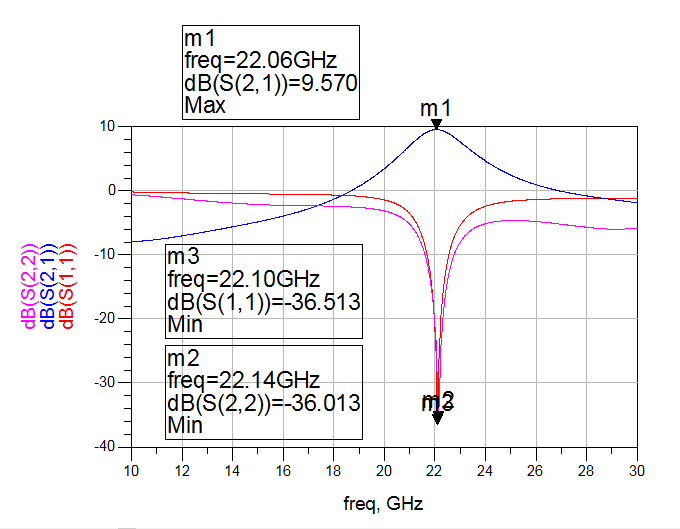
\includegraphics[keepaspectratio=true, scale=0.45]{exps/mf_stub_S}
	\vspace{-0.5em}
	\caption{Parâmetros-S do amplificador com malhas de linhas e stubs.}
	\vspace{-0.8em}
	\label{fig:mf_stub_S}
\end{figure}

Os resultados desta simulação são bastante satisfatórios, no entanto, como foi explicado anteriormente, não será possível utilizar este circuito. Ao observarmos as dimensões dos dispositivos \texttt{MLSC}, reparamos que a sua largura é superior ao seu comprimento, tendo então de representar estes elementos com outros dispositivos, \texttt{MLOC}. Ao dimensionar \texttt{MLOC}, no entanto, o comprimento eléctrico considerado tem de ser incrementado com 90 graus,um exemplo da progressão do processo da dimensão do stub da malha de adaptação pode ser observado na Figura \ref{fig:stub_fail}.

\begin{figure}[H]
	\centering
	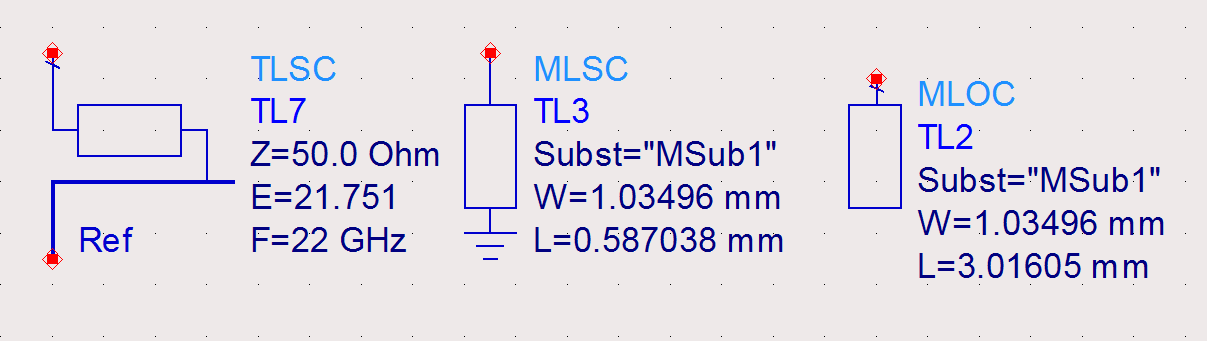
\includegraphics[keepaspectratio=true, scale=0.3]{exps/stub_fail}
	\vspace{-0.5em}
	\caption{Linha ideal - stub - loc}
	\vspace{-0.8em}
	\label{fig:stub_fail}
\end{figure}

\todo{Legenda melhor nesta figura}


\subsection{Concretização do amplificador em tecnologia de microfita}

\subsubsection{a) Introdução de elementos que simulam descontinuidades nas linhas}

\subsubsection{b) Substituição do transístor e condensadores}

\section{Conclusões}

\end{document}